\documentclass{beamer}


\usetheme{Madrid}

\usepackage{booktabs}
\usepackage{siunitx}
\usepackage{graphicx} 
\usepackage{amsmath}
\usepackage{caption}
\usepackage[italian]{babel}
%\usepackage[utf8]{inputenc
\usepackage[absolute,overlay]{textpos}
\usepackage{circuitikz}

\title{Convertitore di impedenza negativa}

% A subtitle is optional and this may be deleted
\subtitle{Studio di un circuito ad "impedenza negativa" realizzato con un op-amp}

\author{S.~Bottaro\inst{1} \and L.M.~Perrone\inst{1}}
% - Give the names in the same order as the appear in the paper.
% - Use the \inst{?} command only if the authors have different
%   affiliation.

\institute[Unipi] % (optional, but mostly needed)
{
  \inst{1}%
  Dipartimento di Fisica\\
  Universita' di Pisa
}
% - Use the \inst command only if there are several affiliations.
% - Keep it simple, no one is interested in your street address.

\date{Recitation - Week04, 2015}

\AtBeginSubsection[]
{
  \begin{frame}<beamer>{Outline}
    \tableofcontents[currentsection,currentsubsection]
  \end{frame}
}

% Let's get started
\begin{document}

\begin{frame}
  \titlepage
\end{frame}

\begin{frame}{Outline}
  \tableofcontents
  % You might wish to add the option [pausesections]
\end{frame}

\section{Convertitore ad impedenza negativa NIC}

\subsection{Analisi del comportamento del circuito}

\begin{frame}

{
\centering
\begin{figure}
\centering
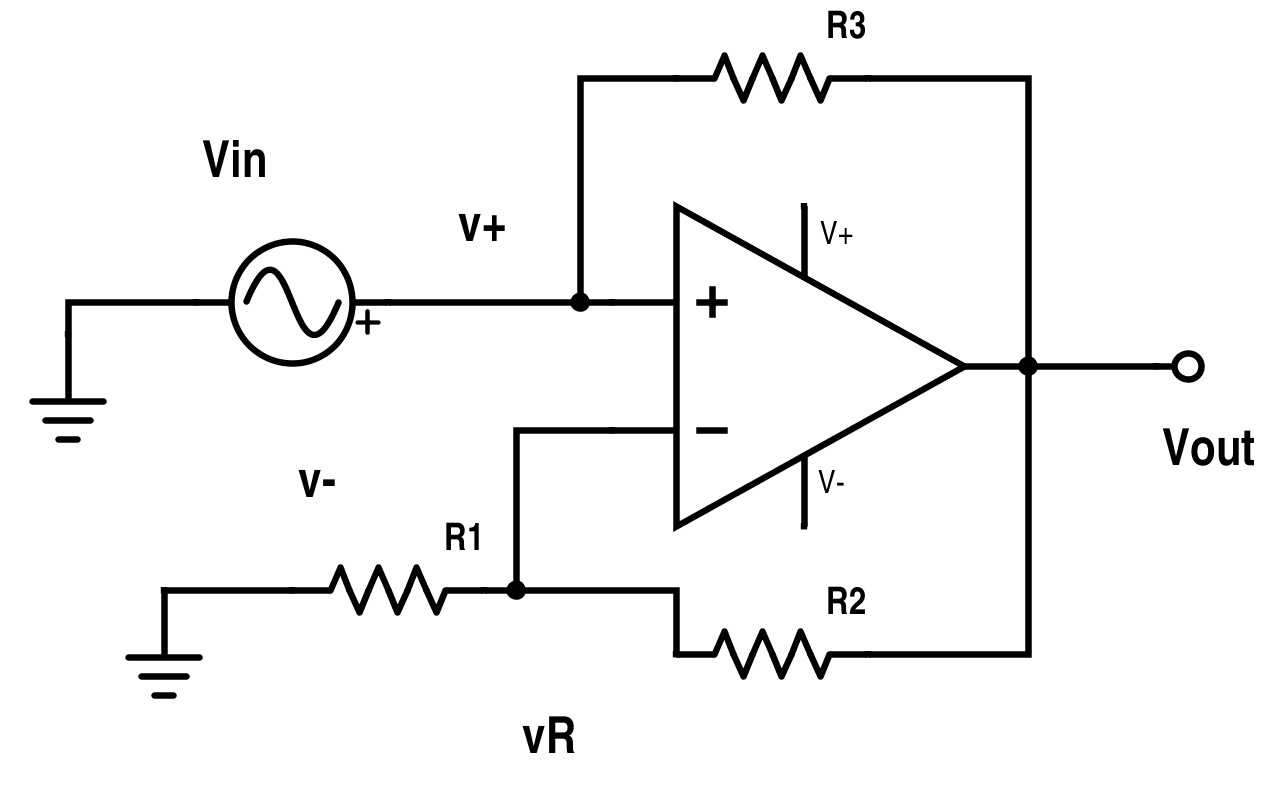
\includegraphics[width=1\linewidth]{./conv-imp-neg}
\caption{Convertitore di impedenza negativa}
\label{fig:conv-imp-neg}
\end{figure}



}

\end{frame}

\begin{frame}{Resistenza equivalente I}
\begin{itemize}
\item Usando le regole d'oro dell'op-amp (non passa corrente nell'integrato, tensione agli ingressi uguale) e' possibile scrivere la resistenza equivalente vista dal generatore:

\item Op-amp in configurazione non-invertente $\Rightarrow$:

\begin{definition}
$V_{out} = V_G (1+\frac{R_2}{R_1})$
\end{definition}

\item Assegnando un verso arbitario antiorario alla corrente che passa per il ramo con $R_3$ $\Rightarrow$:

\begin{definition}
$V_{out} - V_G = R_3 I$
\end{definition}
\end{itemize}
\end{frame}

\begin{frame}
\begin{itemize}

\item Da cui si ottiene:

\begin{theorem}
$V_G = -\frac{R_1 R_3}{R_2}I$
\end{theorem}

Quindi la resistenza equivalente $R$ del circuito e' pari a $R = -\frac{R_1 R_3}{R_2}$, impedenza negativa! (Cioe' la corrente scorre dal nodo $V_{out}$ a $V_G$).
\end{itemize}
\end{frame}

\begin{frame}{Resistenza equivalente II}
\begin{itemize}

\item Nel caso di un generatore reale con resistenza interna $R_G$ possiamo ulteriormente perfezionare la formula precedente operando la sostituzione $V_G \rightarrow V_R = V_G - I\,R_G $, dove $V_R$ e' indicata in figura. Quindi:

\begin{theorem}
$V_G = (R_G - \frac{R_1\, R_3}{R_2})I$
\end{theorem}
\end{itemize}
\end{frame}

\subsection{Simulazioni e progetti di circuito}

\begin{frame}{Come si vede?}
\begin{itemize}
\item Per verificare che quanto visto abbia senso e' possibile procedere in diversi modi:

\begin{itemize}
\item Montare un Ohmetro;
\item Mettere un amperometro in serie a $R_3$;
\item Collegare un voltmetro in parallelo a $R_3$.
\end{itemize}

\item \textsc{attenzione!} La corrente $I$ che passa per la resistenza $R_3$ viene fornita dall'op-amp, quindi il carico complessivo andra' dimensionato in modo tale che questa non superi mai i $25\si{mA}$ di corrente di output del nostro op-amp.
\end{itemize}
\end{frame}

\subsection{Dimensionamento del circuito}

\begin{frame}{Dimensionamento di $R_3$}

{
\centering


\begin{figure}


\begin{tabular}{|c|c|}
\hline 
G -1 & R3 ($ \si{Ohm}$) \\ 
\hline 
10 & 380 \\ 
\hline 
9 & 230 \\ 
\hline 
8 & 150 \\ 
\hline 
7 & 110 \\ 
\hline 
6 & 80 \\ 
\hline 
5 & 60 \\ 
\hline 
\end{tabular} 

\caption{Valori indicativi delle resistenze minime per il corretto funzionamento del circuito in funzione di G, per $V_{in} = 1~V$}
\end{figure}

}

\end{frame}

\begin{frame}

\begin{textblock}{12}(-1,3)
\begin{figure}
\centering
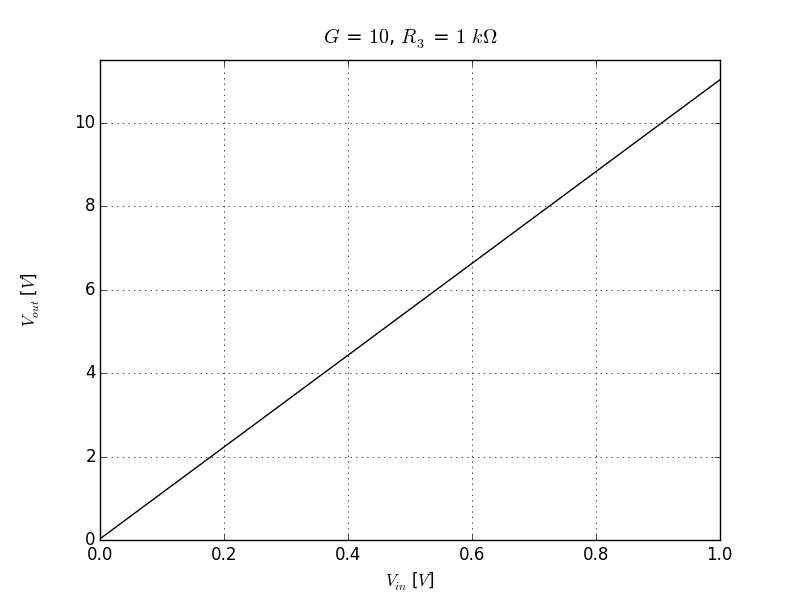
\includegraphics[width=0.6\linewidth]{./g_10_r_1k_dc_v}
\caption{Simulazione del \\
funzionamento a G = 11 e \\
$R_3 = 1k$ ($V_{CC} = \pm 15$)}
\label{fig:bla}
\end{figure}
\end{textblock}


\begin{textblock}{12}(6,3)
\begin{figure}
\centering
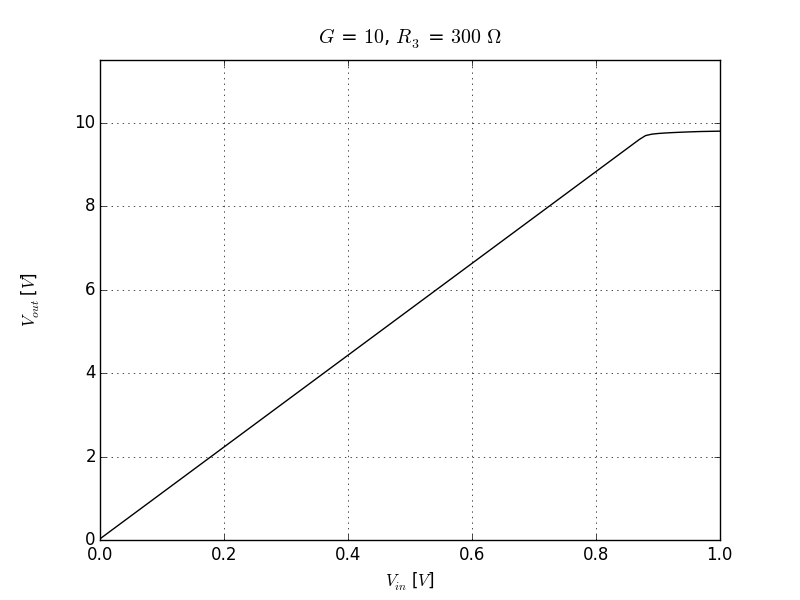
\includegraphics[width=0.6\linewidth]{./g_10_r_300_dc_v}
\caption{Simulazione di \\ 
funzionamento a G = 11 e \\
$R_3 = 300$ ($V_{CC} = \pm 15$)}
\label{fig:prova_gen_10khz_50mpp}
\end{figure}
\end{textblock}



\end{frame}

\begin{frame}{Dimensionamento $R_3$ II}

\begin{figure}
\centering
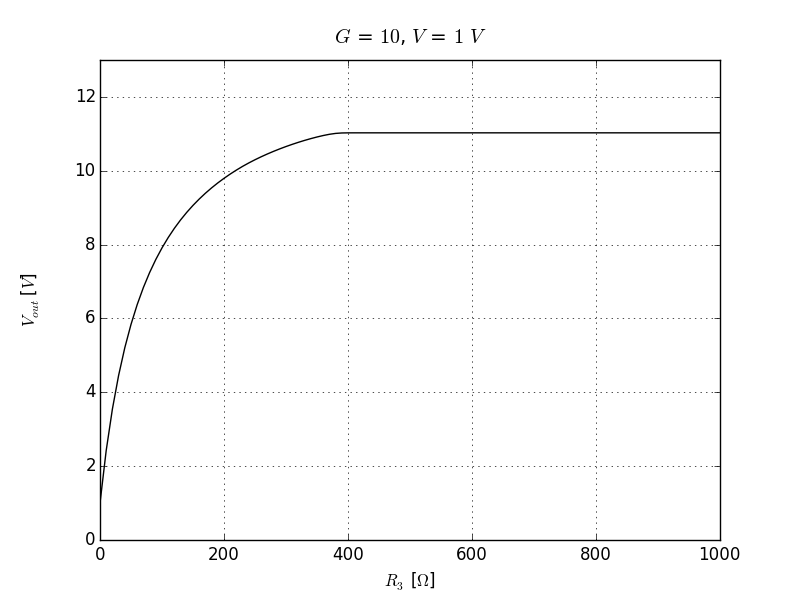
\includegraphics[width=0.7\linewidth]{./g_10_v_1_dc_r}
\caption{Dipendenza di $V_{out} $ da $R_3$ - ipotesi di lavoro}
\label{fig:g_10_v_1_dc_r}
\end{figure}

\end{frame}

\begin{frame}

{
\centering
\begin{figure}
\centering
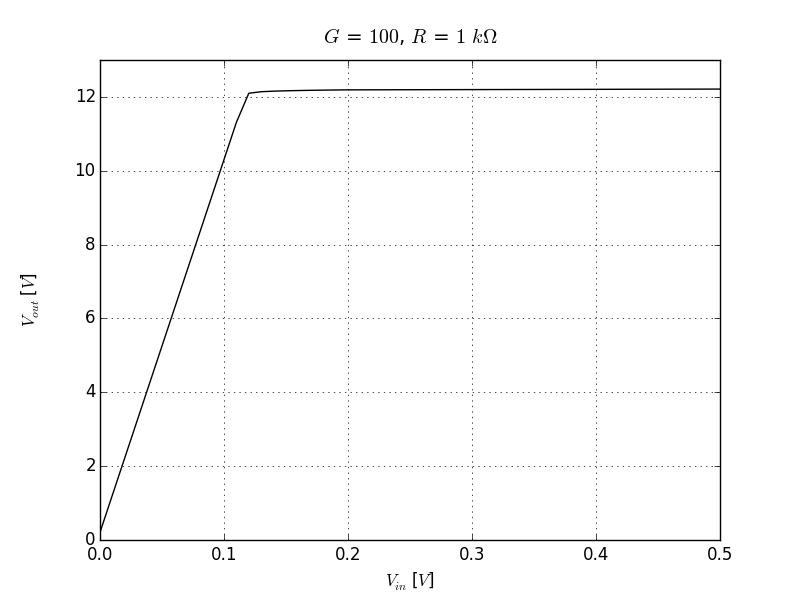
\includegraphics[width=0.7\linewidth]{./g_100_r_1k_dc_v}
\caption{Limite del guadagno in funzione di $V_{in}$}
\label{fig:g_100_r_1k_dc_v}
\end{figure}



}


\end{frame}


\section{Generatore di corrente - Howland Circuit}

\subsection{Analisi del circuito}

\begin{frame}

{
\centering
\begin{figure}
\centering
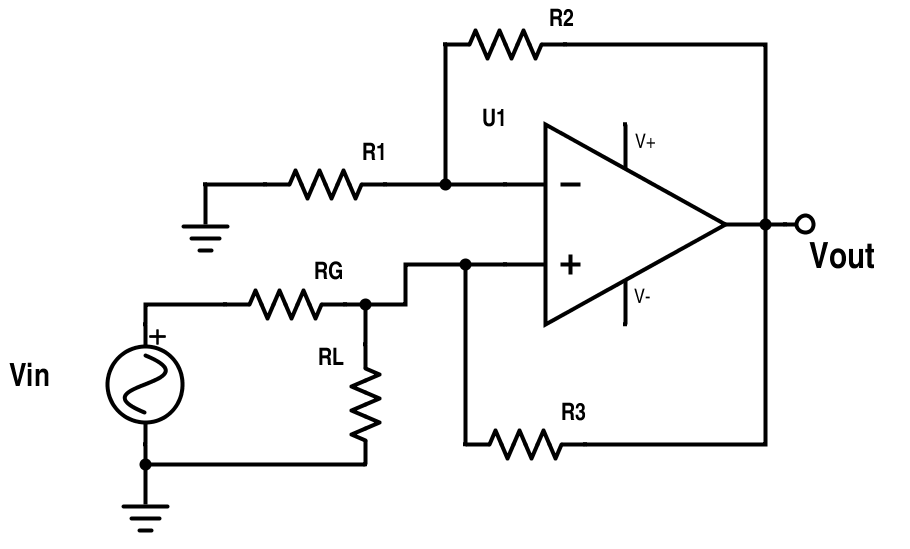
\includegraphics[width=1\linewidth]{./negative-impedance}
\caption{Circuito generatore di corrente}
\label{fig:negative-impedance}
\end{figure}

}
\end{frame}


\begin{frame}{Generatore di corrente}
\begin{itemize}
\item Avendo trovato la resistenza equivalente del convertitore ad impedenza negativa, per risolvere il nuovo circuito possiamo modellizzarlo come un parallelo fra la resistenza di carico $R_L$ e quella equivalente stessa $R_{eq} = -R$.

{
\centering
\begin{figure}
\centering
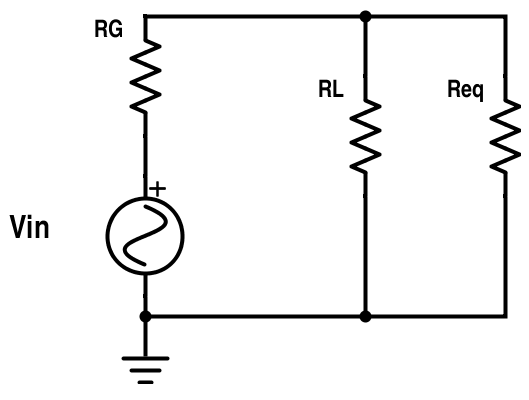
\includegraphics[width=0.6\linewidth]{./neg-resist-equiv}
\caption{Circuito equivalente con R in parallelo}
\label{fig:neg-resist-equiv}
\end{figure}



}


\end{itemize}
\end{frame}

\begin{frame}
\begin{itemize}
\item Risolviamo dunque le equazioni delle maglie:
\begin{definition}
$V_G - R_G \, I_1 - R_L \, I_1 + R_L \, I_2 = 0$
\end{definition}
\begin{definition}
$-R_L \, I_2 + R_L \, I_1 - R_{eq}\,I_2 = 0$
\end{definition}

\item Da cui si ricavano le correnti $I_1$ e $I_2$:
\begin{definition}
$I_1 = \frac{V_G (R_L + R_{eq})}{R_G\,R_L + R_L\,R_{eq} - R_G \, R_{eq}}$
\end{definition}
\begin{definition}
$I_2 = \frac{V_G \,R_L}{R_G\,R_L + R_L\,R_{eq} - R_G \, R_{eq}}$
\end{definition}
\end{itemize}
\end{frame}

\begin{frame}
\begin{itemize}
\item Dato che a noi serve la corrente "netta" che passa per $R_L$, siamo interessati alla differenza $I_L = I_1 - I_2$, con la sostituzione $R_{eq} \rightarrow -R$:

\begin{example}
$I_L = - \frac{V_G \, R}{R_G \, R_L - R_L \, R + R_G \, R}$
\end{example}

Che sotto la condizione $R_G = R$ diventa:

\begin{example}
$I_L = - \frac{V_G}{R}$
\end{example}

Che non dipende da $R_L$!
\end{itemize}
\end{frame}

\subsection{Corrente sul carico}

\begin{frame}

{
\centering

\begin{figure}
\centering
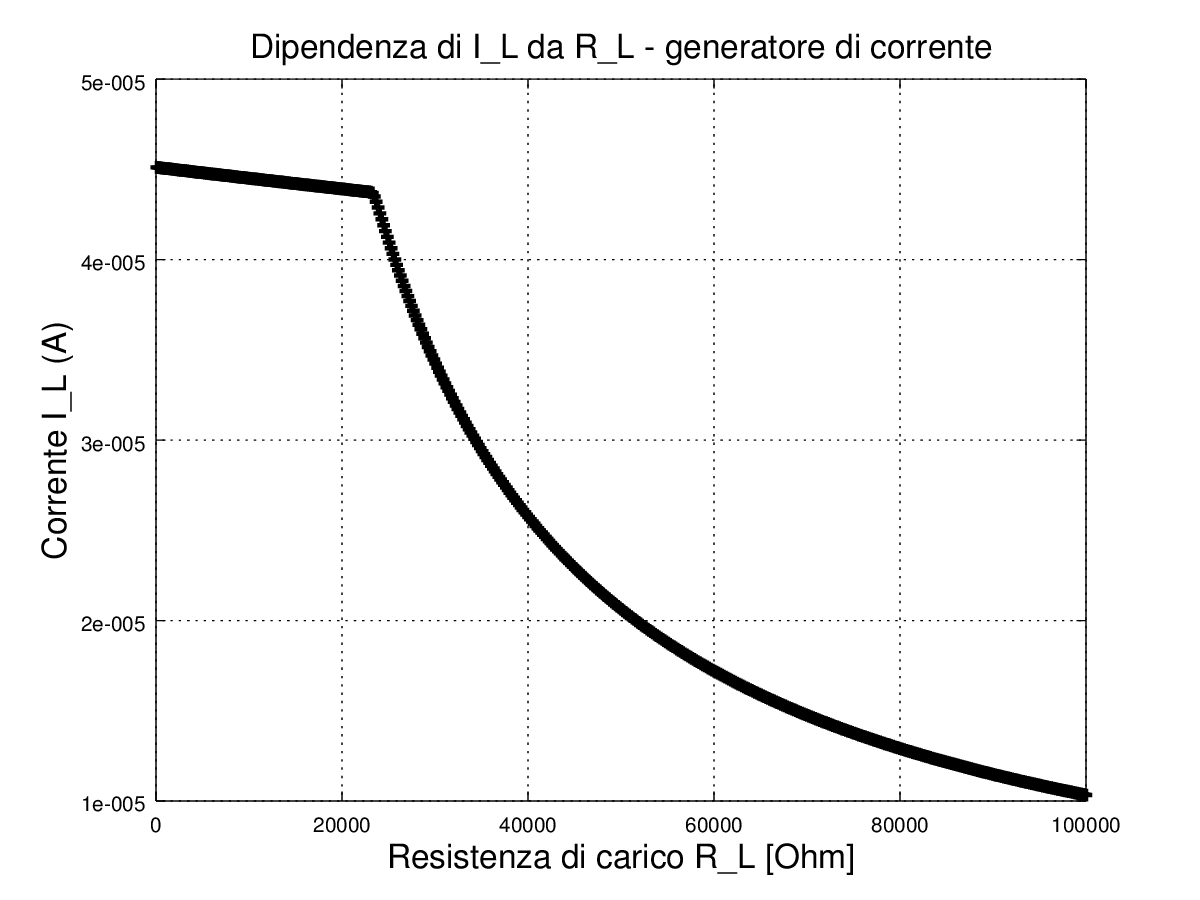
\includegraphics[width=0.7\linewidth]{./corrente_carico_res_carico_R3_500}
\caption{Plot della corrente $I_L$ su resistenza di carico $R_L$ per R3 = 500 Ohm, Vg = 0.5V, R2 = 10k, R1 = 1k, $R_g$ = 50 Ohm}
\label{fig:corrente_carico_res_carico_R3_500}
\end{figure}

}
\end{frame}

\begin{frame}

{
\centering



\begin{figure}
\centering
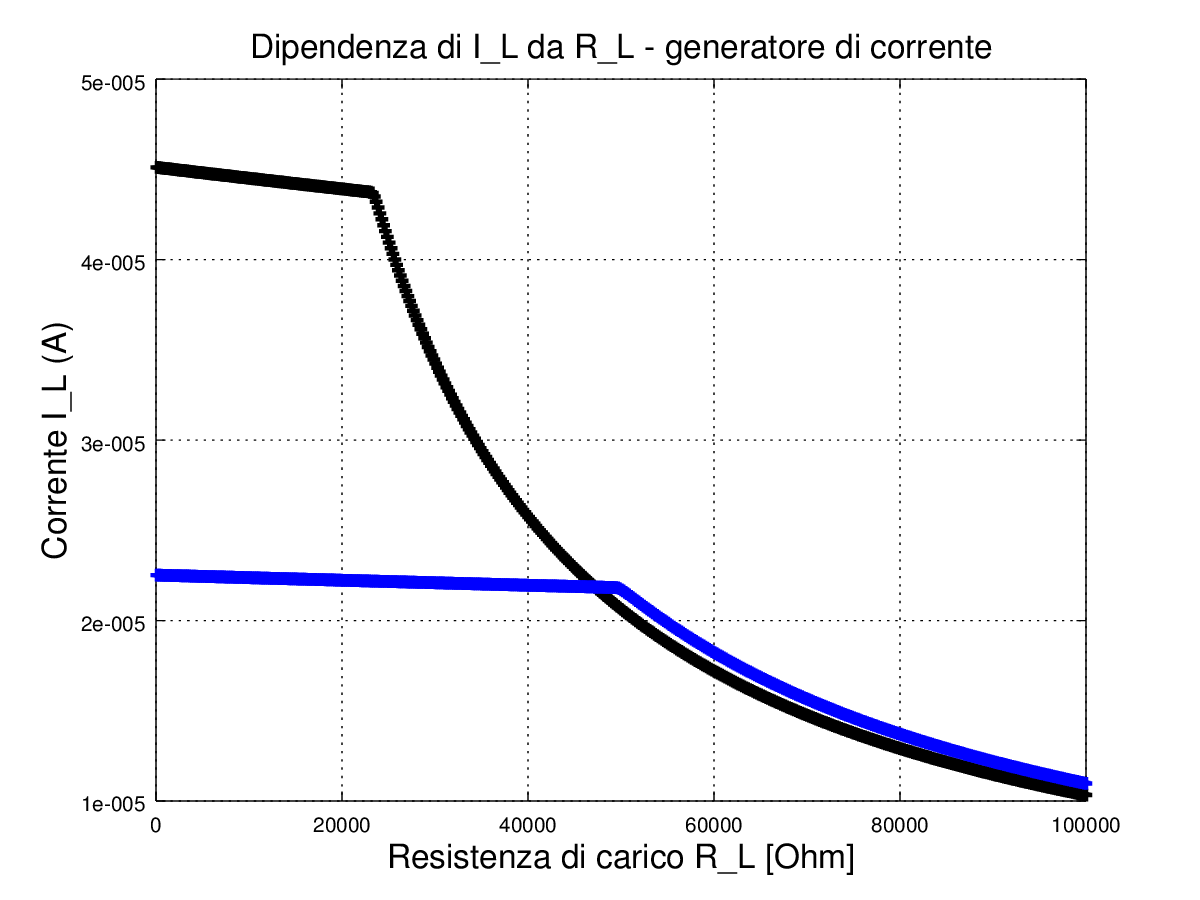
\includegraphics[width=0.7\linewidth]{./corrente_carico_res_carico_R3_500-1k_linear}
\caption{Plot della corrente $I_L$ su resistenza di carico $R_L$, per R3 = 500 Ohm (nero), e R3 = 1k (blu)}
\label{fig:corrente_carico_res_carico_R3_500-1k_linear}
\end{figure}
}
\end{frame}



\begin{frame}

{
\centering

\begin{figure}
\centering
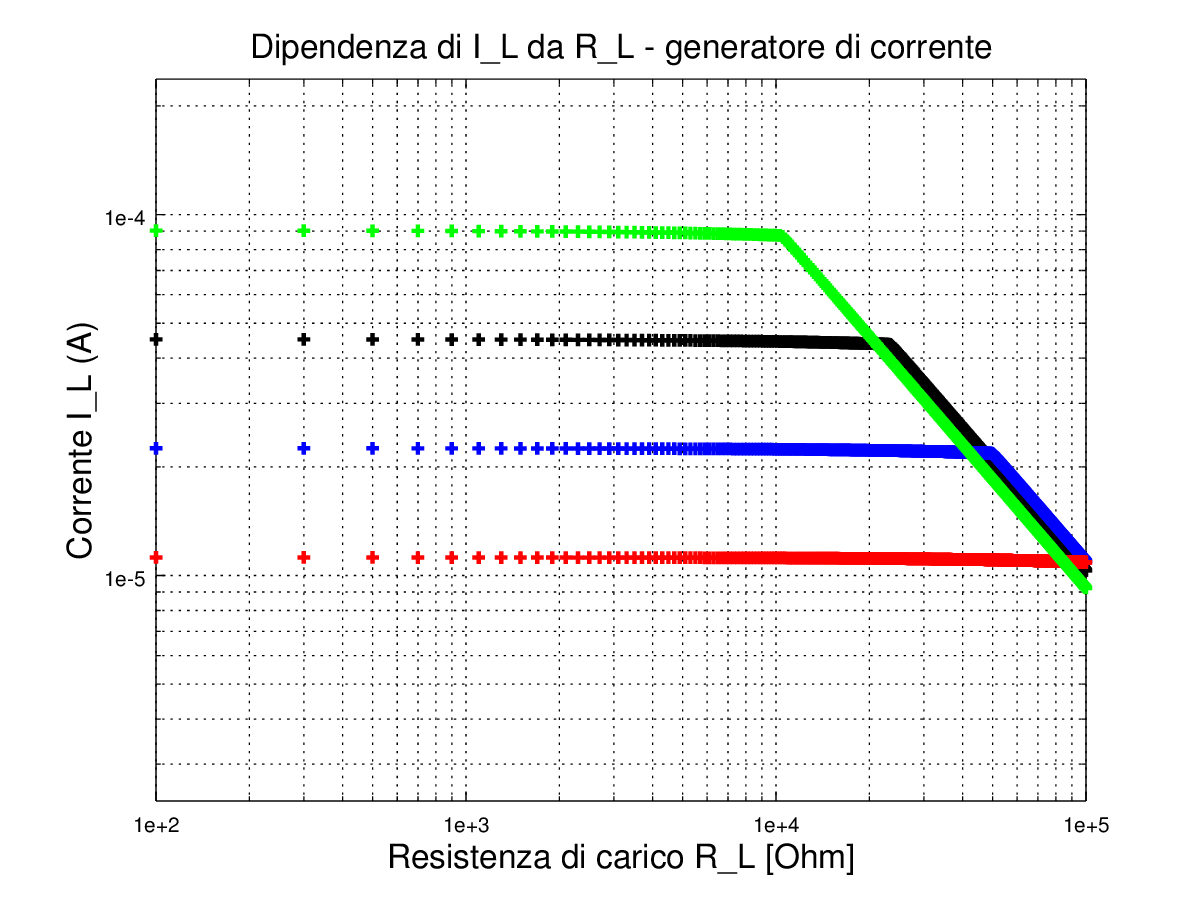
\includegraphics[width=0.7\linewidth]{./corrente_carico_res_carico_R3_500-1k-2k-250_loglog}
\caption{Dipendenza di $I_L$ da $R_L$ - raddoppiamo R3 e $R_G$: R3 = 250 (verde); R3 = 500 Ohm $R_G$ = 50 Ohm (nero); R3 = 1k $R_G$ = 100 Ohm (blu); R3 = 2k $R_G$ = 200 Ohm (rosso)}
\label{fig:corrente_carico_res_carico_R3_500-1k-2k-250_loglog}
\end{figure}



}
\end{frame}



\begin{frame}{Aumentare la regione di \textit{plateau} senza modificare $R_G$}

{
\centering

\begin{figure}
\centering
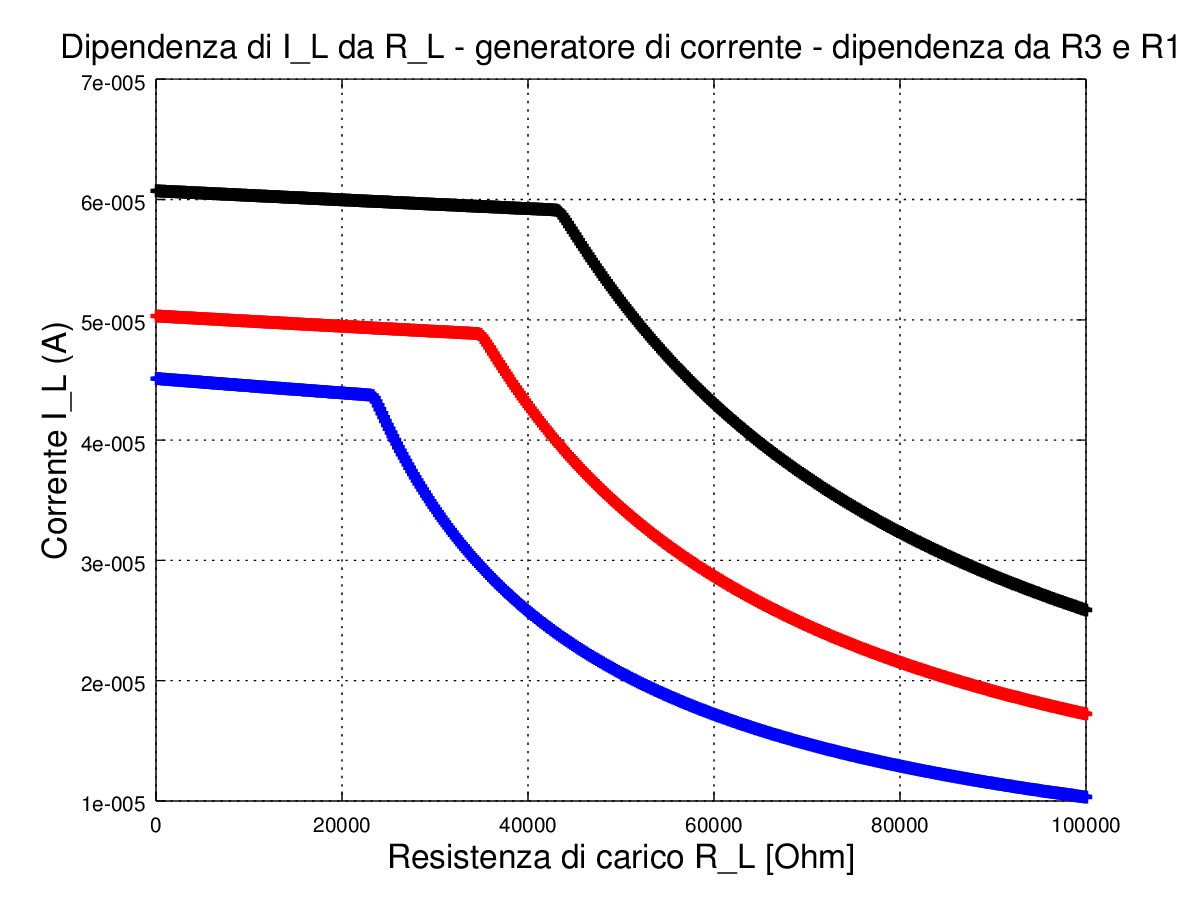
\includegraphics[width=0.7\linewidth]{./corrente_carico_res_carico_R3_125-250-500_R1-4k-2k-1k_linear1}
\caption{$I_L$ su $R_L$: dipendenza da R3 e R1 - raddoppiamo R3 e dimezziamo R1. R3 = 125Ohm, R1 = 4k (nero); R3 = 250 Ohm, R1 = 2k (rosso); R3 = 500 Ohm, R1 = 1k (blu)}
\label{fig:corrente_carico_res_carico_R3_125-250-500_R1-4k-2k-1k_linear1}
\end{figure}


}
\end{frame}

\begin{frame}
\begin{itemize}
\item Troviamo ora la relazione fra la corrente $I_L $ e $V_{out}$. Analizzando il circuito si vede subito che:

\begin{equation}
\begin{cases}
V_L = I_L \, R_L \\
V_{out} = (1+ \frac{R_2}{R_1})V_L
\end{cases}
\end{equation}

\item Per cui:

\begin{definition}
$V_{out} = I_L \, R_L (1+ \frac{R_2}{R_1})$
\end{definition}

Dove $I_L$ (come abbiamo visto) non dipende da $R_L$, quindi c'e' proporzionalita' \underline{lineare}.


\end{itemize}
\end{frame}


\begin{frame}

{
\centering

\begin{figure}
\centering
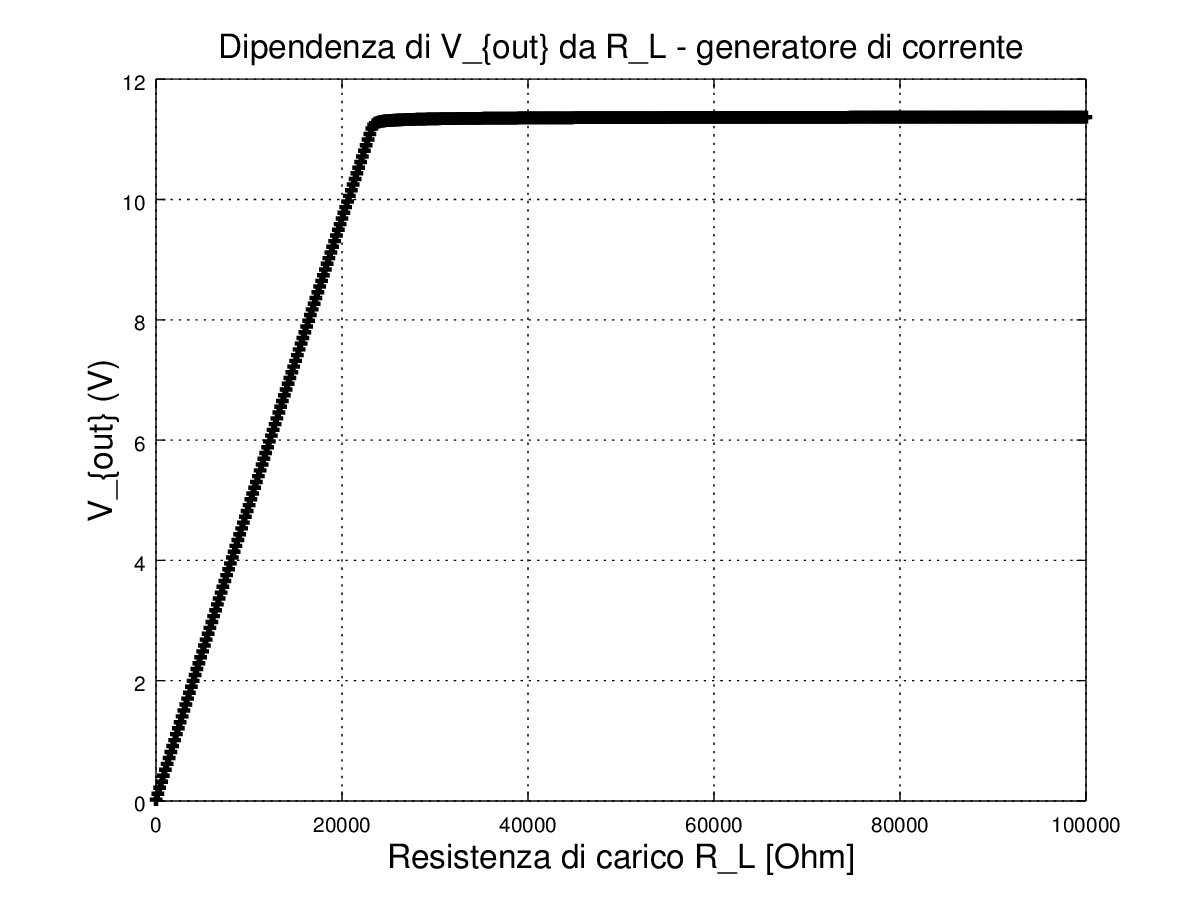
\includegraphics[width=0.7\linewidth]{./Vout_R_L_R3_500}
\caption{$V_{out}$ in funzione di $R_L$ a $R_3 = 500$ fissata, $V_G = 0.5V$}
\label{fig:Vout_R_L_R3_500}
\end{figure}

}
\end{frame}


\begin{frame}

{
\centering
\begin{figure}
\centering
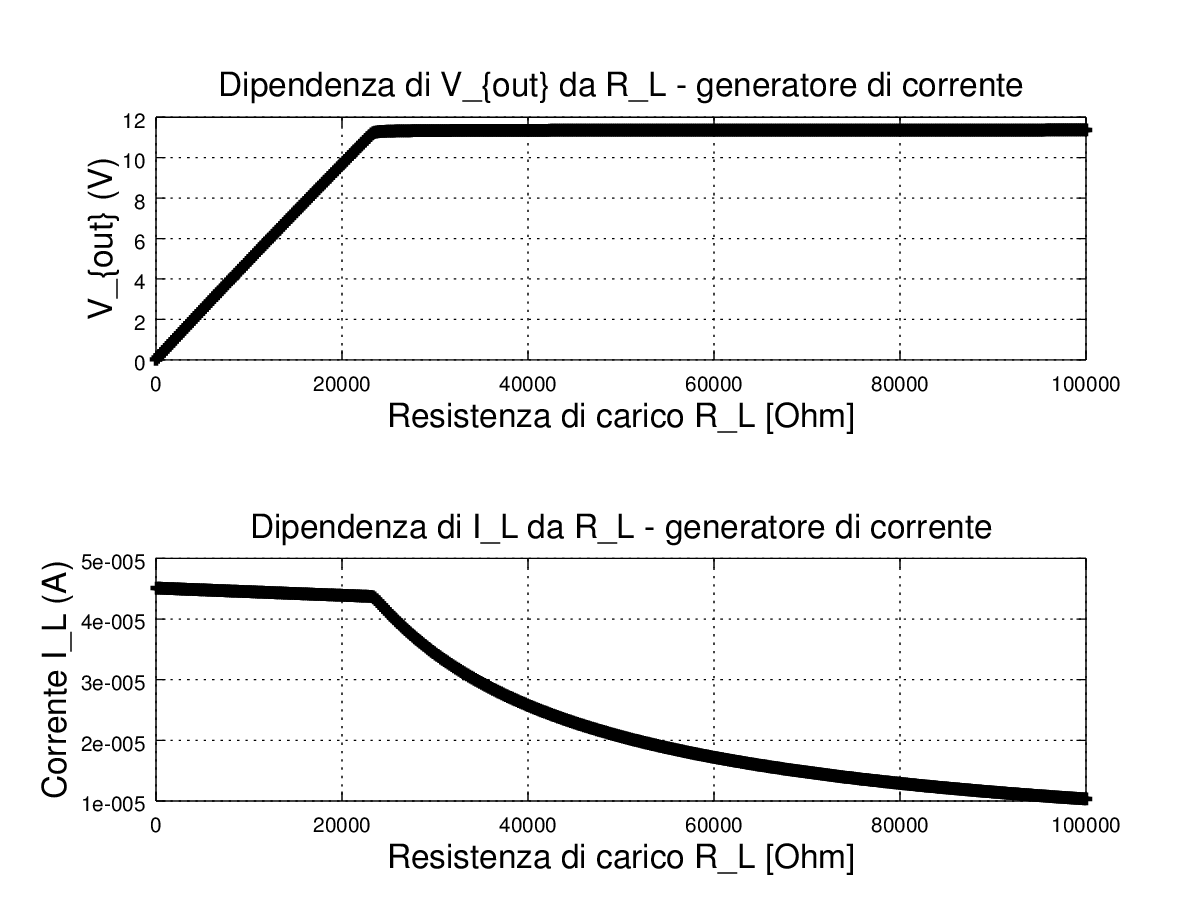
\includegraphics[width=0.7\linewidth]{./Vout_R_L_R3_500_biplot}
\caption{Confronto fra la tensione $V_{out}$ in funzione di $R_L$ e di $I_L$ in funzione di $R_L$ - $R_3 = 500$}
\label{fig:Vout_R_L_R3_500_biplot}
\end{figure}

}
\end{frame}

\begin{frame}{Stima della corrente $I_L$ e del coefficiente angolare}

\begin{itemize}
\item Calcolo del coefficiente angolare della retta:

\begin{definition}
$m_{meas} \simeq 4.8 \, 10^{-4} \, \si{V/ Ohm}$
\end{definition}

In ottimo accordo con quanto previsto dalla relazione: \\


\begin{equation}
V_{out} = I_L \, R_L (1+ \frac{R_2}{R_1})
\end{equation}


Da cui, prendendo la corrente di \textit{plateau} e moltiplicandola per il gain: $ m_{exp} \simeq 4.8 \, 10^{-4} \si{V/ Ohm}$.

\item<2-> {
Ma c'e' un problema!
}

\item<3-> {
Da $I_L = \frac{V_G}{R = R_G} = \frac{0.5 \si{V}}{50 \si{Ohm}} \simeq 10 \si{mA}$ invece di $I_{plateau} \sim 43.8 \, \mu A $.
}

\end{itemize}

\end{frame}

\begin{frame}{A cosa serve?}

\begin{itemize}
\item Generatore di corrente ideale!

\item Generare una differenza di potenziale: la corrente che scorre nel carico RL dipende solo da Vg  quindi la differenza di potenziale ai capi di RL è il segnale Vg per un  fattore RL/R.
\end{itemize}

\end{frame}


\end{document}
